\subsection{Grundlagen der CLT}
\subsection{Versagneskriterium nach Puck}
\subsection{eLamX (T.B.)}
ELamX ist eine Laminatberechnungsprogramm, das anhand der klassischen Laminattheorie mit unterschiedlichen Versagenskriterien berechnen kann, inwiefern ein gewählter Lagenaufbau den Festigkeitskriterien standhält. Zusätzlich sind weitere Funktionen, wie z.B. Beulberechnungen, Optimierungen etc. nutzbar, jedoch für diese Auslegung irrelevant.

\noindent Vorerst wurden die gegeben Materialeigenschaften der Aufgabenstellung als Fasermaterial, Matrixmaterial und  Materialeigenschaften definiert.\\

\begin{tabular}{ll|ll|ll}
	\multicolumn{2}{c}{Fasermaterial} &\multicolumn{2}{c}{Matrixmaterial}  &\multicolumn{2}{c}{Materialeigenschaften} \\
	\hline
	$\rho_{f}$ & $2,55 \frac{g}{cm^{3}}$  & $\rho_{m}$ & $1,18 \frac{g}{cm^{3}}$  & $R_{\parallel}^{+}$ & $597,9MPa$ \\
	\hline
	$E_{f,11}$ & $74000MPa$  & $E_{M}$ & $3300MPa$  & $R_{\parallel}^{-}$ & $650,0MPa$\\
	\hline
	$E_{f,22}$ & $74000MPa$  & $G_{M}$ & $1222MPa$  & $R_{\perp}^{+}$ & $37,7MPa$\\
	\hline
	$G_{f,12}$ & $30800MPa$ & $\nu_{M}$ & $0,35$  & $R_{\perp}^{+-}$ & $130,0MPa$\\
	\hline
	$\nu_{f,21}$ & $0,2$  & &   & $R_{\parallel\perp}$ & $37,5MPa$\\
\end{tabular}\\

\noindent Mit einem Faservolumenanteil $\varphi=0,4$ ergeben sich folgende weitere Materialeigenschaften:\\

\begin{tabular}{ll}
	$\rho$ & $1,728 \frac{g}{cm^{3}}$ \\
	\hline
	$E_{\parallel}$ & $31580 MPa$\\
	\hline
	$E_{\perp}$ & $5341,2MPa$\\
	\hline
	$\nu_{\parallel\perp}$ & $0,29$\\
	\hline
	$G_{\parallel\perp}$ & $1984,5 MPa$\\
\end{tabular}\\

\noindent Anschließend werden die nach Kapitel ? (VDI 2013) berechneten Laminate bzw. Lagenzusammensetzungen aus aus mehreren Material-Lagen zusammengesetzt. Eine Gewebelage wird dabei durch zwei einzelne Materiallagen mit einem Winkel von $90°$ zueinander simuliert, sodass sich die doppelte Anzahl des Materials gegenüber der Lagenanzahl ergibt.Für die Holmgurte ergibt sich ein Lagenaufbau nach \~{ref:Lagenaufbau Holmgurte} und für den dünnen Steg nach \~{ref:Lagenaufbau Steg dünn}. FÜe den dicken Steg ergibt sich der gleich Aufbau wie bei dem dünnen Steg, allerdings mit 24 Lagen. Weshalb die sich die Anzahl der Gewebelagen gegenüber der Auslegung nach [VDI 2013] unterscheidet, wird folgend beschrieben.\\ 

\begin{figure}
	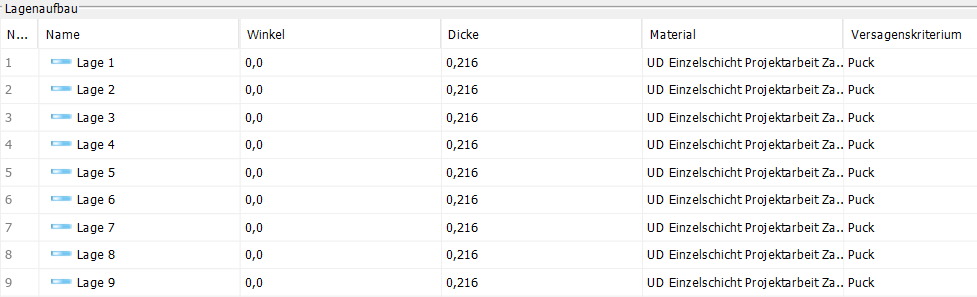
\includegraphics[width=1.0\textwidth]{Bilder/Lagenaufbau Holmgurte.png}
	\caption{Lagenaufbau Holmgurte}
	\label{fig:Lagenaufbau Holmgurte}
\end{figure}
\begin{figure}
	\includegraphics[width=1.0\textwidth]{Bilder/Lagenaufbau Steg dünn.png}
	\caption{Lagenaufbau Steg dünn}
	\label{fig:Lagenaufbau Steg dünn}
\end{figure}
\noindent Anschließend werden 